%!TEX root = ../thesis.tex

\chapter[a brief overview of unsupervised neural speech representation learning]{A Brief Overview of Unsupervised Neural Speech Representation Learning}
\label{app:paper-brief}
\ifthenelse{\equal{\skipappendices}{true}}{}{

\section*{Abstract}
Unsupervised representation learning for speech processing has matured greatly in the last few years. Work in computer vision and natural language processing has paved the way, but speech data offers unique challenges. As a result, methods from other domains rarely translate directly. We review the development of unsupervised representation learning for speech over the last decade. We identify two primary model categories: self-supervised methods and probabilistic latent variable models. We describe the models and develop a comprehensive taxonomy. Finally, we discuss and compare models from the two categories.


\section{Introduction}
Representation learning has shaped modern computer vision \cite{simonyan_very_2014} and natural language processing \cite{devlin_bert_2018}, and more recently speech processing has been subject to the same development \cite{baevski_wav2vec_2020}. Representation learning has been defined as \emph{``learning representations of the data that make it easier to extract useful information when building classifiers or other predictors"} \cite{bengio_representation_2013}.  
Unsupervised representation learning is concerned with learning useful representations without the use of human annotations. Usually, a model is first pre-trained on a task where plenty of data is available. The model is then fine-tuned, or used to extract input representations for a smaller model, targeting a task with limited training data. In computer vision, both supervised \cite{simonyan_very_2014, szegedy_going_2015, he_deep_2015} and unsupervised \cite{pathak_context_2016, doersch_unsupervised_2015} representation learning have gained attention with supervised representation learning driven by the availability of large annotated datasets \cite{deng_imagenet_2009}. For text and speech, pre-training is usually unsupervised as labeled data is difficult to obtain. Although work on text has paved the way, and the two fields share many characteristics, learning representations from speech is a problem faced with a unique set of challenges.

In this paper, we survey work on unsupervised representation learning for speech processing from within the last decade.
From a methodological perspective, we identify two primary model categories, namely models based on self-supervised learning and probabilistic latent variable models. 
We provide a methodological review of the design choices related to each of the model categories and develop a model taxonomy that highlights the different directions of work. Finally, we compare and discuss models from the two categories and their respective evaluation procedures.

\begin{figure}[!t]
    \begin{flushleft}
        \textsc{\small \hspace{0.16\textwidth} self-supervised \hspace{0.22\textwidth} latent variable}
    \end{flushleft}
    \centering
    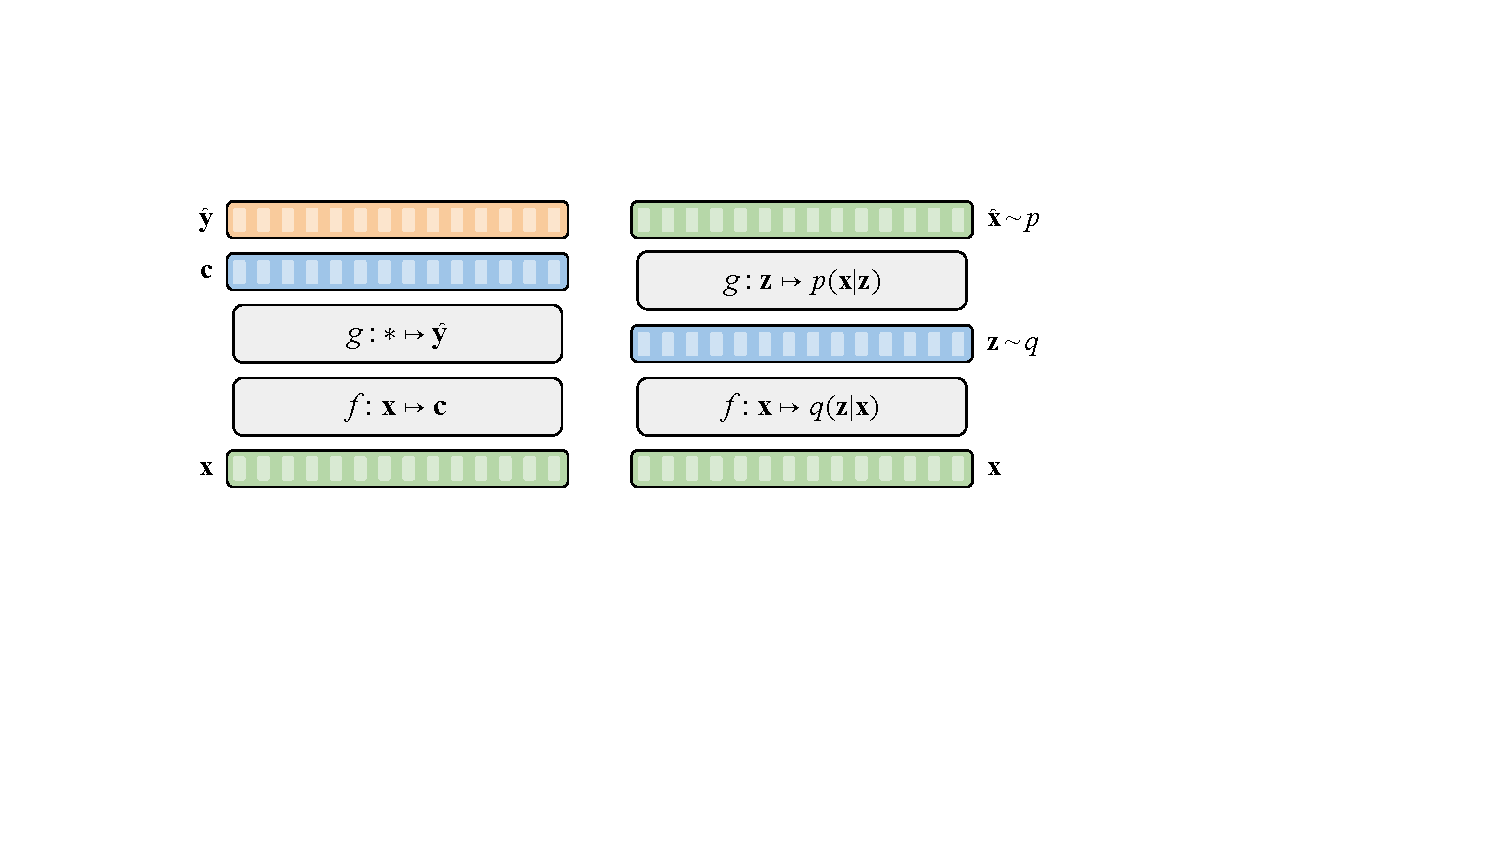
\includegraphics[width=0.90\textwidth]{paper_brief/SSL_LVM.pdf}
    \caption{A schematic overview of the two groups of models covered in this survey. \textit{Left}: A model trained with self-supervised learning. We take these models to consist of two functions $f(\cdot)$ and $g(\cdot)$ (\cref{ssec:notation}). After pre-training, $f(\cdot)$ is fine-tuned or used for extracting features $\mathbf{c}$. $g(\cdot)$ is an auxiliary function used to accommodate the self-supervised pre-training task. \textit{Right}: A probabilistic latent variable model. In contrast to the self-supervised model, the functions $f(\cdot)$ and $g(\cdot)$ learn the parameters of distributions $q$ and $p$. The latent variable $\mathbf{z}$ is commonly used for representation learning.}
    \label{fig:ssl_lvm}
\end{figure}

\section{Unsupervised representation learning}\label{ssec:notation}

In the following, we group previous work into \textit{self-supervised models} and \textit{probabilistic latent variable models}, and take a \emph{model} to comprise a neural architecture and a corresponding learning algorithm. A schematic overview is found in \cref{fig:ssl_lvm}. These categories are neither exhaustive nor mutually exclusive, but allow us to focus on the characteristics that have shaped different branches of research. 

With emphasis on recent successes in the field, we cover literature from the last 10 years. While a complete description of all relevant models is not within the scope of this work, we sketch important technicalities when they are particularly descriptive of certain models. We first define our high-level notation and conventions to ease discussion.

\paragraph{Notation}
We use the subscript $i{:}j$ with $i{\leq}j$ to denote a vector sequence $\textbf{a}_{i:j}$ containing elements $\textbf{a}_{i}$ through $\textbf{a}_{j}$. We denote model input as $\mathbf{x}_{1:T}$ which, in practice, might be either a spectrogram or the raw speech signal, but we do not distinguish between the two in notation as it is not essential to understand the models. Also, models commonly downsample the temporal dimension, but again, this is not crucial to understand the models, so we maintain a notation based on a single temporal dimension $t\in\{1,\dots, T\}$.

When discussing self-supervised models, we use $\mathbf{c}_{1:T}$ to denote a contextualized representation. For stochastic latent variable models, we use $\mathbf{z}_{1:T}$ as is customary to the field. 
While some models are frozen and produce representations used as input for downstream tasks (\textbf{\textsc{frz}}, \cref{tab:model-taxonomy}), others are designed to be fine-tuned (\textbf{\textsc{ftn}}, \cref{tab:model-taxonomy}). In either case, we use $f(\cdot)$ to denote the model that is used for the downstream task. We use $g(\cdot)$ to denote any auxiliary model components (e.g., for a reconstruction task we might have $g: \mathbf{c}_t \mapsto \hat{\mathbf{x}}_t$). When a model can be naturally subdivided into multiple components, we simply use $f_*(\cdot)$ where $*$ may be any convenient descriptor. Finally, we often use a subscript when defining a loss, $\mathcal{L}_i$, to imply that the total loss is computed as a sum over $i$.


\subsection{Self-supervised models}
\label{sec:ssmodels}

Self-supervised learning is a subset of unsupervised learning \cite{tsai_selfsupervised_2021}. Where other unsupervised methods can be seen as a means to an end in itself (e.g., clustering or data generation), self-supervised learning takes the form of a pretext task that only adds value when associated with a downstream task. This makes self-supervised learning tie naturally with semi-supervised learning, but it may also be part of a fully unsupervised setup \cite{baevski_unsupervised_2021}. Self-supervised learning is often characterized by automatically deriving the target from the input or other unlabeled examples \cite{ouali_overview_2020}.

\paragraph{Predictive models}
Similar to classic autoregressive language models \cite{mikolov_recurrent_2010}, contextualized speech representations can be learned by predicting future values of a simple representation \cite{oord_representation_2018, chung_unsupervised_2019, schneider_wav2vec_2019, chung_generative_2020, jiang_further_2021} (\textbf{\textsc{prd}}, \cref{tab:model-taxonomy}). Modeling spectrograms directly, autoregressive predictive coding (APC, \citealp{chung_unsupervised_2019}) is perhaps the simplest example in this category. The forward pass and loss are computed as
\begin{align}
    \mathbf{c}_{t} &= f(\mathbf{x}_{1:t})  \label{eq_brief:apc_f} \\ 
    \hat{\mathbf{x}}_{t+k} &= g(\mathbf{c}_{t}) \\
    \mathcal{L}_t &= \lVert \hat{\mathbf{x}}_{t+k} - \mathbf{x}_{t+k} \rVert_1\enspace.
\end{align}
%
\noindent Here, $f(\cdot)$ and $g(\cdot)$ are parameterized by neural networks such that each $\mathbf{c}_t$ is only conditioned on previous inputs $\mathbf{x}_{1:t}$ and $\hat{\mathbf{x}}_{t+k}$ is computed step-wise. \citet{chung_unsupervised_2019} use a stack of unidirectional LSTMs for $f(\cdot)$ and a linear regression layer for $g(\cdot)$. Tasks that seek to predict or reconstruct the input are very common. In the literature, these are often jointly referred to as reconstruction tasks (\textbf{\textsc{rec}}, \cref{tab:model-taxonomy}) \cite{liu_tera_2021, wang_unispeech_2021}, although this is somewhat misleading in the case of prediction.

Contrary to generative models, such as WaveNet \cite{oord_wavenet_2016}, the APC model is not restricted to next-step prediction. Instead, it predicts $k > 0$ steps ahead in order to ensure that the model does not learn a trivial solution by exploiting the smoothness of the signal. Depending on the downstream task, we are often interested in learning so-called slow features that will typically span multiple input frames \cite{wiskott_slow_2002}. Even the smallest linguistic units of speech, phonemes, tend to span $0.1$ seconds on average \cite{garofolo_timit_1993}, whereas spectrogram frames $\mathbf{x}_t$ are typically computed at $0.01$ second intervals. However, sometimes local smoothness is explicitly used to define the task \cite{badino_autoencoder_2014, jati_speaker2vec_2017, jati_neural_2019}.

\paragraph{Contrastive models}
Speech contains localized noise (e.g., phase shifts) that does not inform slow feature learning. Thus, directly modeling speech might not be the best way to learn contextualized representations. Contrastive predictive coding (CPC,  \citealp{oord_representation_2018}) targets a local variable $\mathbf{v}_{1:T}$, learned from the model input $\mathbf{x}_{1:T}$, instead of the input itself. The forward pass is
%
\begin{align}
    \mathbf{v}_{t} &= f_{v}(\mathbf{x}_{t-r:t+r}) \label{eq_brief: cpc local representation} \\
    \mathbf{c}_{t} &= f_{c}(\mathbf{v}_{1:t}) \\
    \hat{\mathbf{v}}_{t,k} &= g_k(\mathbf{c}_{t}) \enspace,
\end{align}
%
\noindent where $f_v(\cdot)$ is a convolutional neural network, such that each $\mathbf{v}_{t}$ only encodes information from a limited receptive field $2r+1$. Again, $f_c(\cdot)$ should be limited to condition each $\mathbf{c}_t$ on previous time-steps $\mathbf{v}_{1:t}$ and $g_k(\cdot)$ is a step-wise transformation. The loss is based on noise constrastive estimation \cite{gutmann_noisecontrastive_2010} and is given by
\begin{align}
    \mathcal{L}_{t,k} &= - \log \left(\frac{\exp(\hat{\mathbf{v}}_{t,k}^{\text{\tiny T}}\mathbf{v}_{t+k})}{\sum_{n \sim \mathcal{D}} \exp(\hat{\mathbf{v}}_{t,k}^{\text{\tiny T}}\mathbf{v}_{n})} \right)\enspace .
    \label{eq_brief: cpc loss}
\end{align}
%
\noindent Here, $\mathcal{D}$ is a set of indices including the target index $t+k$ and negative samples drawn from a proposal distribution, which is typically taken to be a uniform distribution over the set $\{1,\dots,T\}$. Note that the loss is also indexed by $k$ to show that CPC targets multiple offsets. The APC model is easily extended in a similar way \cite{chung_improved_2020}.

Crucially, we cannot simply predict $\mathbf{v}_{t+k}$ from $\mathbf{c}_t$ with an $\ell_1$ loss. This would cause $f_v(\cdot)$ to collapse to a trivial solution, such as setting all $\mathbf{v}_t$ equal. With a contrastive loss on the other hand, setting all $\mathbf{v}_t$ equal would cause $\mathcal{L}_{k,t}$ to be constant at a value no better than a random baseline. 

A model closely related to the original CPC model is wav2vec \cite{schneider_wav2vec_2019}. It uses a different parameterization of the functions $f_v(\cdot)$ and $f_c(\cdot)$, and modifies the loss to consider a binary prediction task, such that we have
%
\begin{align}
    \mathcal{L}_{t,k} &= - \log(\sigma(\hat{\mathbf{v}}_{t,k}^{\text{\tiny T}}\mathbf{v}_{t+k})) - \sum_{n \sim \mathcal{D}} \log(\sigma(-\hat{\mathbf{v}}_{t,k}^{\text{\tiny T}}\mathbf{v}_{n})) \,.
    \label{eq_brief: wav2vec loss}
\end{align}

\noindent This model was among the first to show that learned representations can be used to improve end-to-end speech recognition. As we will see, the wav2vec framework has evolved to shape state-of-the-art representation learning for speech.


\paragraph{Masking-based models} One downside of predictive tasks is that models are primarily unidirectional. Some work has extended APC and CPC inspired models with separate encoders operating in opposite directions \cite{ling_deep_2020, kawakami_learning_2020, borgholt_scaling_2021}, but these models are still restricted to process left and right context separately. Inspired by the masked language model task used for text-based representation learning \cite{devlin_bert_2018}, several papers have used masking to overcome this challenge (\textbf{\textsc{msk}}, \cref{tab:model-taxonomy}). Masking refers to replacing parts of the input with zeros or a learned masking vector. For zero-masking \cite{jiang_improving_2019, liu_mockingjay_2020, wang_unsupervised_2020, chi_audio_2020, ling_decoar_2020}, we have
\begin{align}
    \mathbf{c}_{1:T} &= f(\mathbf{x}_{1:T} \circ \mathbf{m}_{1:T})\\
    \mathbf{\hat{x}}_{t} &= g(\mathbf{c}_{t}) \\
    \mathcal{L}_t &= \lVert \mathbf{\hat{x}}_{t} - \mathbf{x}_{t} \rVert_1\enspace,
\end{align}
where the $\circ$ operator denotes the Hadamard product, $f(\cdot)$ is typically a transformer encoder or a bidirectional recurrent neural network, $g(\cdot)$ is a step-wise transformation, and $\mathbf{m}_{1:T}$ is a mask such that $m_{t,i} \in \{0,1\}$. Alternatively, $\mathbf{m}_{1:T}$ is used to select which $\mathbf{x}_t$ are replaced by a learned masking vector. The entries of $\mathbf{m}_{1:T}$ are determined by some stochastic policy. One frequent inspiration is SpecAugment \cite{park_specaugment_2019}, which was originally proposed for supervised speech recognition and applies frequency and time masking to spectrogram representations.
While temporal masking is most common, frequency masking has also been adopted for representation learning  \cite{wang_unsupervised_2020}. A simple, yet popular, masking strategy is to draw a proportion of input indices $t_i\sim\{1,\dots,T-M\}$ without replacement, and then mask $\{t_i, \dots, t_i+M\}$ \cite{baevski_wav2vec_2020, hsu_hubert_2021, ling_decoar_2020}.

Combining masking with a contrastive loss, wav2vec 2.0 was the first work to show that a competitive speech recognition model can be learned by fine-tuning a pre-trained model with as little as 10 minutes of labeled data. For this model
%
\begin{align}
    \mathbf{v}_{t} &= f_v(\mathbf{x}_{t-r:t+r}) \\
    \mathbf{c}_{1:T} &= f_c(\mathbf{v}_{1:T} \circ \mathbf{m}_{1:T}) \\
    \mathbf{q}_t &= g_q(\mathbf{v}_t) \enspace . \label{eq_brief: w2v2 qtz}
\end{align}

\noindent Here, $f_v(\cdot)$ is a convolutional neural network, $f_c(\cdot)$ is a transformer encoder \cite{vaswani_attention_2017} and $g_q(\cdot)$ is a quantization module used to learn targets from the localized variable $\mathbf{v}_{1:T}$. Computing quantized targets this way requires an extra loss term, which we will present when we discuss quantization in general below. The contrastive loss for wav2vec 2.0 is similar to that of the CPC model,
%
\begin{align}
    \mathcal{L}_t &= - \log \left(\frac{\exp(S_{\text{c}}(\mathbf{c}_{t}, \mathbf{q}_{t}))}{\sum_{n \sim \mathcal{D}} \exp(S_{\text{c}}(\mathbf{c}_{t}, \mathbf{q}_{n}))} \right) \enspace , \label{eq_brief: w2v2 loss}
\end{align}
%
\noindent where $S_{\text{c}}(\cdot)$ is the cosine similarity and the negative samples in $\mathcal{D}$ are sampled from other masked time-steps. 

In general, masking is less data efficient than prediction, as only the masked portion of the input is non-trivial to reconstruct. For this reason, the loss might be computed as
%
\begin{align}
    \mathcal{L}_t &= \lVert (\mathbf{\hat{x}}_{t} - \mathbf{x}_{t}) \circ (\mathbf{1} - \mathbf{m}_t) \rVert_1 \enspace .
\end{align}

\noindent Non-autoregressive predictive coding (NPC, \citealp{liu_nonautoregressive_2020}) tries to resolve this by using a convolutional neural network where the kernel is masked instead of the input.
This allows for complete data utilization, but limits the amount of context encoded in the learned representation.
\cref{fig:ssl_grid} summarizes the models discussed so far.

\begin{figure}[!t]
    \centering
    \setlength\tabcolsep{1.5pt}
    \begin{tabular}{>{\centering\arraybackslash} m{4mm}  >{\centering\arraybackslash} m{0.40\textwidth}|>{\centering\arraybackslash} m{0.40\textwidth}}
          & {\small \textsc{predictive}} & {\small \textsc{masking-based}} \\
        \rotatebox{90}{{\small \textsc{reconstruct}}} & 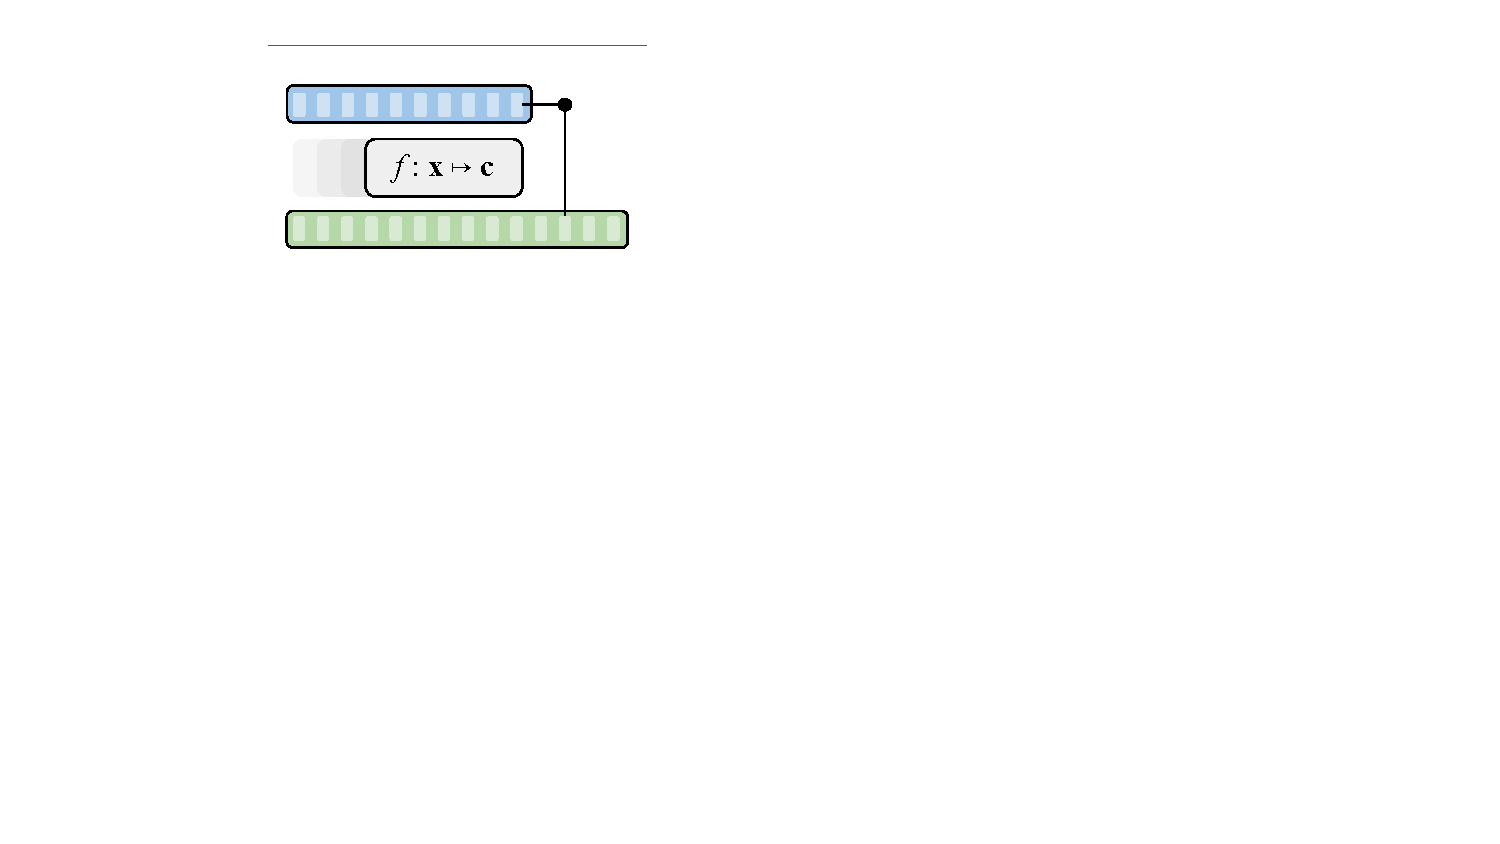
\includegraphics[width=0.40\textwidth]{paper_brief/REC_PRD.pdf} & 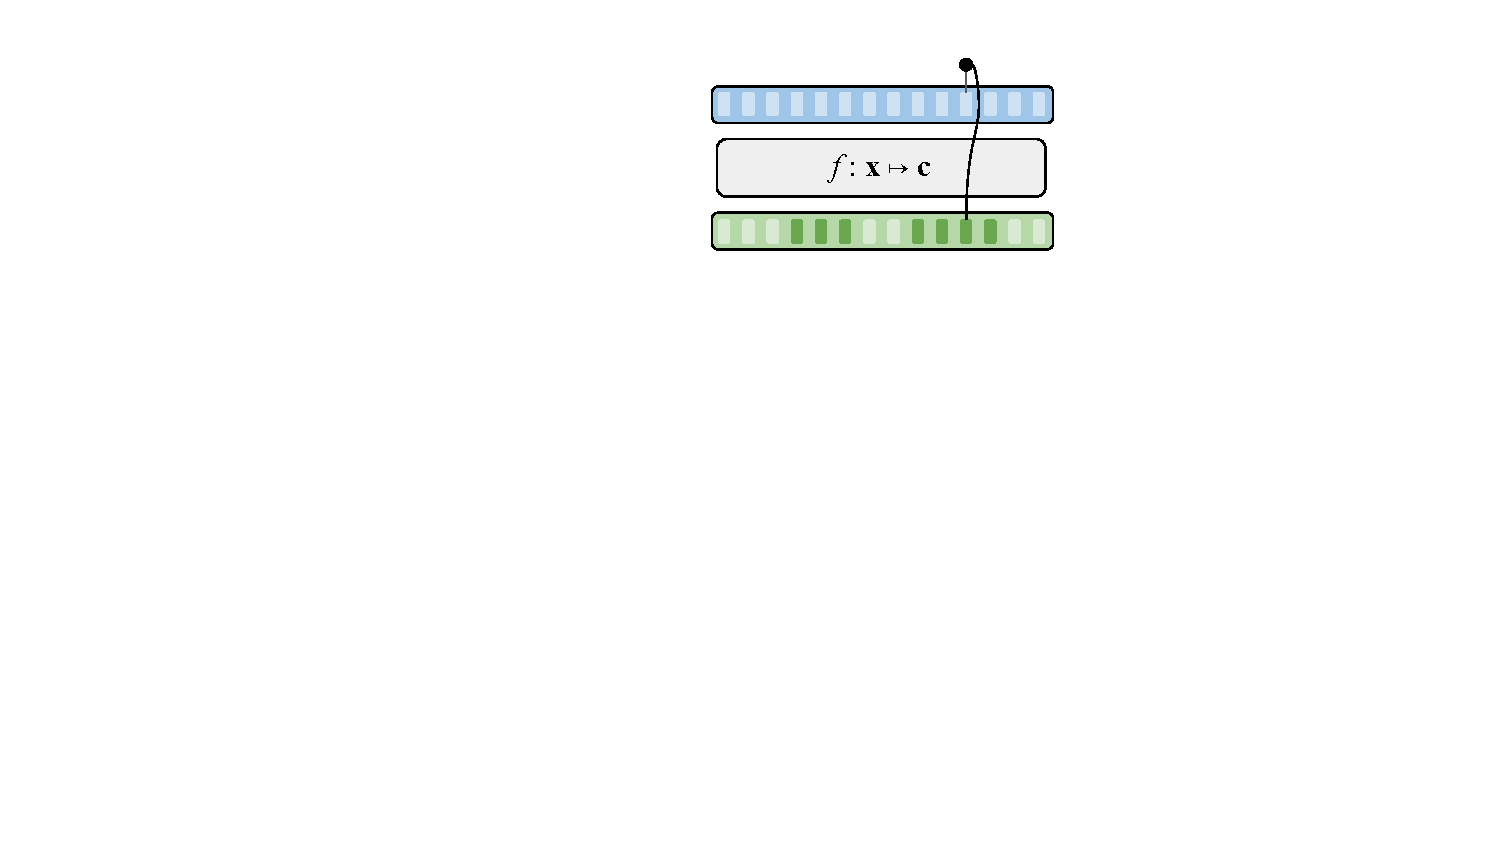
\includegraphics[width=0.40\textwidth]{paper_brief/REC_MSK.pdf}  \\
        \midrule
        \rotatebox{90}{{\small \textsc{contrastive}}} & 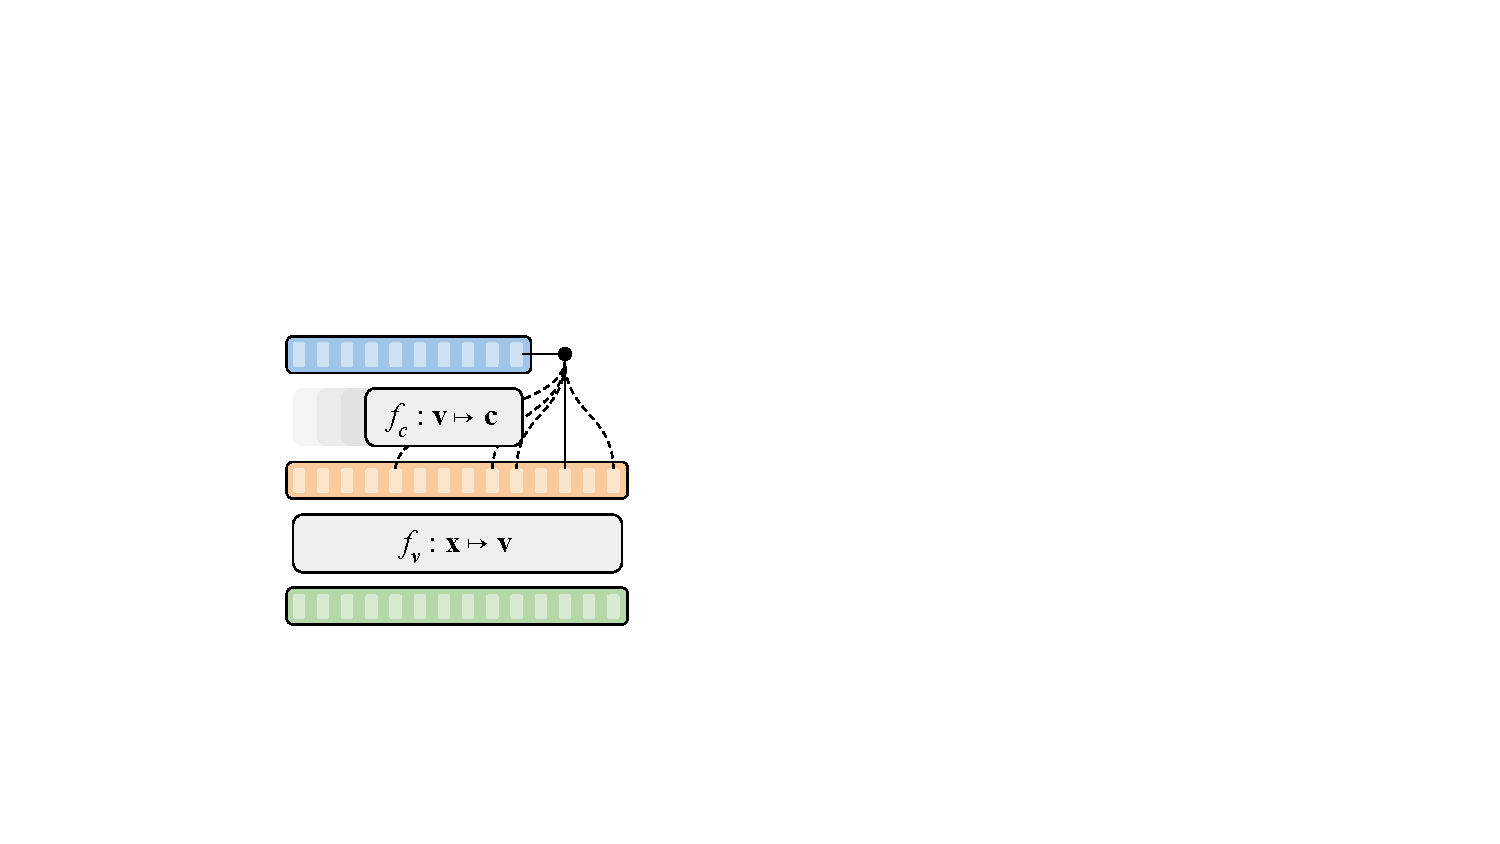
\includegraphics[width=0.40\textwidth]{paper_brief/CON_PRD.pdf} & 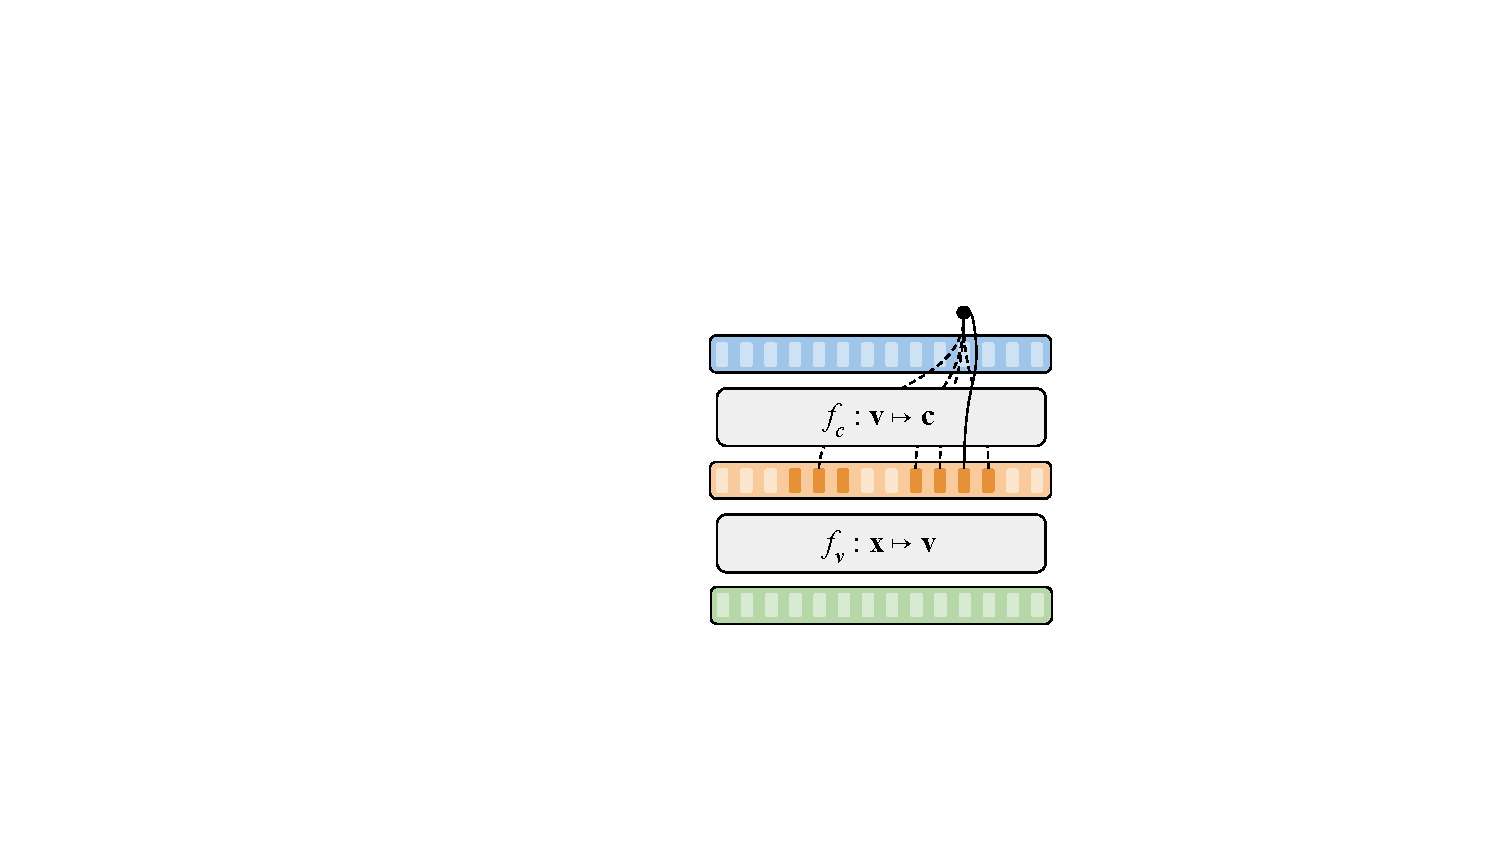
\includegraphics[width=0.40\textwidth]{paper_brief/CON_MSK.pdf}
    \end{tabular}
    \caption{Schematic of self-supervised methods. Each subfigure illustrates the loss computation for a single time-step. The temporal subscript has been left out for simplicity.}
    \label{fig:ssl_grid}
\end{figure}



\begin{sidewaystable*}[t]
    \caption{Selected models classified according to the binary attributes identified throughout the text. The models are sorted according to first publication date on arXiv which might differ from the citation year. \textbf{\textsc{msk}}: masking, \textbf{\textsc{prd}}: prediction, \textbf{\textsc{con}}: contrastive, \textbf{\textsc{rec}}: reconstruction, \textbf{\textsc{qtz}}: quantization, \textbf{\textsc{gen}}: generative, \textbf{\textsc{frz}}: frozen, \textbf{\textsc{ftn}}: fine-tuned, \textbf{\textsc{loc}}: local, \textbf{\textsc{glo}}: global.}
    \label{tab:model-taxonomy}
    \begin{center}
        \renewcommand{\arraystretch}{1.1}
        \resizebox{0.925\textwidth}{!}{%
        \begin{tabular}{ l l | c c c c c c | c c c | c c } 
            \toprule
            
            \multicolumn{2}{c}{} & 
            \multicolumn{6}{c}{\footnotesize\textsc{Model and task design}} & 
            \multicolumn{3}{c}{\footnotesize\textsc{Resolution}} &
            \multicolumn{2}{c}{\footnotesize\makebox[0pt][c]{\textsc{Usage}}} \\
            \textbf{\textsc{model}} &
            \textbf{\textsc{pub. date}} &
            \textbf{\textsc{msk}} & 
            \textbf{\textsc{prd}} & 
            \textbf{\textsc{con}} &  
            \textbf{\textsc{rec}} &  
            \textbf{\textsc{qtz}} & 
            \textbf{\textsc{gen}} & 
            \textbf{\textsc{loc}} & 
            \textbf{\textsc{glb}} & 
            \textbf{\textsc{var}} & 
            \textbf{\textsc{frz}} & 
            \textbf{\textsc{ftn}} \\
            
            \midrule
            \multicolumn{12}{c}{\textsc{Self-supervised models}} \\
            \midrule
            %                                                           MSK      PRD      CON      REC      QTZ      GEN      LOC      GLB     VAR      FRZ      FTN
            \textbf{Audio Word2vec} \footnotesize\cite{chung_audio_2016}      & 2016 Mar. & \cmark & \xmark & \xmark & \cmark & \xmark & \xmark & \xmark & \cmark & \xmark & \cmark & \xmark \\
            \textbf{Speech2Vec} \footnotesize\cite{chung_speech2vec_2018}     & 2018 Mar. & \xmark & \cmark & \xmark & \cmark & \xmark & \xmark & \xmark & \cmark & \xmark & \cmark & \xmark \\
            \textbf{Unspeech} \footnotesize\cite{milde_unspeech_2018}         & 2018 Apr. & \xmark & \cmark & \cmark & \xmark & \xmark & \xmark & \xmark & \cmark & \xmark & \cmark & \xmark \\
            
            \textbf{CPC} (van den Oord et al. 2018)         & 2018 Jul. & \xmark & \cmark & \cmark & \xmark & \xmark & \xmark & \cmark & \xmark & \xmark & \cmark & \xmark \\
            
            \textbf{APC} \footnotesize\cite{chung_unsupervised_2019}          & 2019 Oct. & \xmark & \cmark & \xmark & \cmark & \xmark & \xmark & \cmark & \xmark & \xmark & \cmark & \xmark \\ % 5/4
            \textbf{wav2vec} \footnotesize\cite{schneider_wav2vec_2019}       & 2019 Apr. & \xmark & \cmark & \cmark & \xmark & \xmark & \xmark & \cmark & \xmark & \xmark & \cmark & \xmark \\ % 11/4
            \textbf{Mockingjay}  \footnotesize\cite{liu_mockingjay_2020}      & 2019 Oct. & \cmark & \xmark & \xmark & \cmark & \xmark & \xmark & \cmark & \xmark & \xmark & \cmark & \cmark \\ % 25/10-19
            \textbf{wav2vec 2.0} \footnotesize\cite{baevski_wav2vec_2020}     & 2020 Jun. & \cmark & \xmark & \cmark & \xmark & \cmark & \xmark & \cmark & \xmark & \xmark & \xmark & \cmark \\ % 20/6
            \textbf{NPC} \footnotesize\cite{liu_nonautoregressive_2020}                     & 2020 Nov. & \cmark & \xmark & \xmark & \cmark & \cmark & \xmark & \cmark & \xmark & \xmark & \cmark & \xmark \\ % 1/11
            \textbf{DeCoAR 2.0} \footnotesize\cite{ling_decoar_2020}          & 2020 Dec. & \cmark & \xmark & \xmark & \cmark & \cmark & \xmark & \cmark & \xmark & \xmark & \cmark & \xmark \\ % 11/12
            \textbf{SCPC} \footnotesize\cite{bhati_segmental_2021}            & 2021 Jun. & \xmark & \cmark & \cmark & \xmark & \xmark & \xmark & \cmark & \xmark & \cmark & \cmark & \xmark \\ % 3/6
            \textbf{HuBERT} \footnotesize\cite{hsu_hubert_2021}               & 2021 Jun. & \cmark & \xmark & \xmark & \xmark & \cmark & \xmark & \cmark & \xmark & \xmark & \xmark & \cmark \\ % 14/6
            \midrule
            \multicolumn{12}{c}{\textsc{Probabilistic latent variable models}} \\
            \midrule
            %                                                           MSK      PRD      CON      REC      QTZ      GEN      LOC      GLO     VAR      FRZ      FTN
            \textbf{VRNN} \footnotesize\cite{chung_recurrent_2015}          & 2015 Jun. & \xmark & \xmark & \xmark & \cmark & \xmark & \cmark & \cmark & \xmark & \xmark & \cmark & \xmark \\
            \textbf{SRNN} \footnotesize\cite{fraccaro_sequential_2016}      & 2016 May  & \xmark & \xmark & \xmark & \cmark & \xmark & \cmark & \cmark & \xmark & \xmark & \cmark & \xmark \\
            \textbf{HMM-VAE} \footnotesize\cite{ebbers_hidden_2017}         & 2017 Mar. & \xmark & \xmark & \xmark & \cmark & \xmark & \cmark & \cmark & \xmark & \xmark & \cmark & \xmark \\
            \textbf{ConvVAE} \footnotesize\cite{hsu_learning_2017}          & 2017 Apr. & \xmark & \xmark & \xmark & \cmark & \xmark & \cmark & \xmark & \cmark & \xmark & \cmark & \xmark \\
            \textbf{FHVAE} \footnotesize\cite{hsu_unsupervised_2017}        & 2017 Sep. & \xmark & \xmark & \xmark & \cmark & \xmark & \cmark & \cmark & \cmark & \xmark & \cmark & \xmark \\
            \textbf{VQ-VAE} (van den Oord et al. 2018)                      & 2017 Nov. & \xmark & \xmark & \xmark & \cmark & \cmark & \cmark & \cmark & \xmark & \xmark & \cmark & \xmark \\
            \textbf{BHMM-VAE} \footnotesize\cite{glarner_full_2018}         & 2018 Mar. & \xmark & \xmark & \xmark & \cmark & \xmark & \cmark & \cmark & \xmark & \xmark & \cmark & \xmark \\
            \textbf{STCN} \footnotesize\cite{aksan_stcn_2019}               & 2019 Feb. & \xmark & \xmark & \xmark & \cmark & \xmark & \cmark & \cmark & \xmark & \xmark & \cmark & \xmark \\
            \textbf{FDMM} \footnotesize\cite{khurana_factorial_2019}        & 2019 Oct. & \xmark & \xmark & \xmark & \cmark & \xmark & \cmark & \cmark & \cmark & \xmark & \cmark & \xmark \\
            \textbf{ConvDMM} \footnotesize\cite{khurana_convolutional_2020} & 2020 Jun. & \xmark & \xmark & \xmark & \cmark & \xmark & \cmark & \cmark & \xmark & \xmark & \cmark & \xmark \\
            \bottomrule
        \end{tabular}
        }
    \end{center}
\end{sidewaystable*}
    

\paragraph{Quantization} 
Several models enforce a discrete latent space by quantizing the vector representation (\textbf{\textsc{qtz}}, \cref{tab:model-taxonomy}). The two most popular approaches are the Gumbel-softmax \cite{jang_categorical_2016, maddison_concrete_2017} and the quantization used in the VQ-VAE \cite{oord_neural_2018}.

\textit{Gumbel-softmax approach:} 
Say we want to quantize a vector $\mathbf{v}$ such that it takes one of $K$ possible values. We first map $\mathbf{v}$ to $\mathbf{l} \in \mathbb{R}^K$ and then map $\mathbf{l}$ to a probability vector $\mathbf{p} \in \mathbb{R}^K$ via the Gumbel softmax given by
\begin{align}
    p_i &= \frac{\exp(l_i + n_i) / \tau}{\sum_k^K \exp(l_k + n_k) / \tau} 
\end{align}
for $i=1,\dots,K$. Here $\tau$ is a temperature parameter and $\mathbf{n}\in\mathbb R^K$ is a random vector with $n_i = -\log(-\log(u_i))$ for $u_i \sim \mathcal{U}(0, 1)$.
As  $\tau \rightarrow 0$, $\mathbf{p}$ approaches a one-hot vector. The Gumbel noise $\mathbf{n}$ is a practical way to sample from the untempered categorical distribution (i.e., $\tau = 1$).
$\mathbf{p}$ is mapped to a one-hot vector using a function $\varphi(\cdot)$, such that $\varphi(\mathbf{p})_i = 1$ if $i = \argmax_j p_j$ and $0$ otherwise. 
As this function is non-differentiable, we must rely on the straight-through gradient estimator \cite{bengio_estimating_2013} which assumes that the Jacobian ${\partial \, \varphi}/{\partial \, \mathbf{p}}$ equals the identity matrix. 
The one-hot vector can then be used for a codebook lookup to obtain the final quantized vector (e.g., $\mathbf{q}_t$ in \cref{eq_brief: w2v2 qtz}).

The wav2vec 2.0 quantization module (\cref{eq_brief: w2v2 qtz}) uses the Gumbel softmax. To ensure utilization of codebook vectors, a diversity loss is added to the task specific loss (\cref{eq_brief: w2v2 loss})
%
\begin{align}
    \mathcal{L} =  - H(\widetilde{\mathbf{p}}) / K \enspace,
\end{align}
\noindent where $H(\cdot)$ is the entropy and $\widetilde{\mathbf{p}}$ is the untempered version of $\mathbf{p}$ without Gumbel noise.

\textit{VQ-VAE approach:} Instead of directly parameterizing a probability distribution, as in the Gumbel softmax, a vector $\mathbf{v}$ can be quantized by replacing it with the closest codebook vector $\mathbf{e}_k$. Specifically, given a learned codebook $\mathbf{e}\in\mathbb{R}^{K\times D}$, where $K$ is the codebook size and $D$ is the dimensionality of each codebook vector $\mathbf{e}_k$, the quantized representation $\mathbf{q}$ of $\mathbf{v}$ is obtained as,
\begin{align}
    \mathbf{q} = \mathbf{e}_k \ , \enspace \text{where} \enspace k=\arg\min_j \norm{\mathbf{v} - \mathbf{e}_j}_2 \enspace .
\end{align}
As $\arg\min$ is non-differentiable, the straight-through estimator is used as for the Gumbel-softmax. 
Codebook learning is facilitated by a two-term auxiliary loss similar to classical vector quantization dictionary learning \cite{burton_generalization_1983, soong_vector_1985}. Gradients for the codebook vectors are given solely by a vector quantization term. A so-called commitment term ensures that non-quantized vectors do not grow unboundedly.
\begin{align}
    \mathcal{L} = \underset{\text{vq}}{\underbrace{\norm{\text{sg}\left[\mathbf{v}\right] - \mathbf{e}}_2^2}} + \underset{\text{commitment}}{\underbrace{\beta\norm{\mathbf{v} - \text{sg}\left[\mathbf{e}\right]}_2^2}} \enspace , \label{eq_brief: vector quantization losses}
\end{align}
where $\text{sg}[\mathbf{x}] = \mathbf{x}$ is the stop-gradient operator with the property $\frac{d}{dx_i}\text{sg}[\mathbf{x}] \equiv 0$ for all $i$ and $\beta$ is a hyperparameter. Although vector quantization was introduced by the VQ-VAE which is, in some ways, a latent variable model, it has been applied to self-supervised methods \cite{vanniekerk_vectorquantized_2020, baevski_vqwav2vec_2020}.

\textit{Motivation:} Similar to how quantization approaches differ between works, so do the motivations provided for employing them. The vq-wav2vec \cite{baevski_vqwav2vec_2020, baevski_effectiveness_2020} learn quantized representations in order to apply natural language processing models, like BERT \cite{devlin_bert_2018}, afterwards. Other works use quantization for speech segmentation \cite{kamper_unsupervised_2021, chorowski_unsupervised_2019} or as a bottleneck in order to ``\textit{limit model capacity}" \cite{chung_vectorquantized_2020, ling_decoar_2020}.
Finally, \citet{chung_vectorquantized_2020} explore quantization between different layers in the APC model, but find that continuous representations consistently perform better than their quantized counterparts on a downstream phoneme classification task

Given our previous discussion of how it might not be beneficial to model localized noise, quantization in wav2vec 2.0 seems well motivated, as it enforces the target representation $\mathbf{q}_{1:T}$ to discard such noise. Taking this idea further, the HuBERT model \cite{hsu_hubert_2021} uses offline quantization to learn categorical targets. Initially, spectrogram features are used to learn frame-wise labels with $k$-means clustering. A model similar to wav2vec 2.0, but without online quantization, is then trained to infer labels for masked time-steps. Since quantization is offline, this model does not need to rely on a contrastive loss, but can infer the target class directly. The offline quantization also ensures more stable training, as targets do not change abruptly.


\paragraph{Global representations}
The models covered so far learn representations that maintain a temporal resolution proportional to the input resolution. We say that they learn local representations (\textbf{\textsc{loc}}, \cref{tab:model-taxonomy}). Now, we cover models that learn global representations (\textbf{\textsc{glb}}, \cref{tab:model-taxonomy}).
 
Early work on global speech representation learning takes inspiration from the autoencoder framework \cite{kramer_nonlinear_1991}. \citet{chung_audio_2016} propose a simple sequence-to-sequence autoencoder for learning acoustic word embeddings:
\begin{align}
    \mathbf{c} &= f(\mathbf{x}_{1:T}) \\
    \hat{\mathbf{x}}_{1:T} &= g(\mathbf{c}) \enspace , \label{eq_brief:dec-aw2v}
\end{align}

\noindent where $f(\cdot)$ and $g(\cdot)$ are a recurrent neural networks, such that $\mathbf{c}$ is taken to be the hidden state at the last time-step $T$ of $f(\cdot)$ and used as initial hidden state of $g(\cdot)$. 
The authors also propose a denoising autoencoder with masked inputs $f(\mathbf{x}_{1:T} \circ \mathbf{m}_{1:T})$. Similar RNN-based autoencoders have also been explored \cite{kamper_truly_2019, holzenberger_learning_2018}.

Prior to this work, \citet{kamper_unsupervised_2015} and \citet{renshaw_comparison_2015} introduced the \textit{correspondence autoencoder}. This method uses dynamic time warping to align input-target segment pairs extracted with unsupervised term discovery. In more recent work, the need for alignment has been alleviated by adopting the sequence-to-sequence framework \cite{kamper_truly_2019, jacobs_acoustic_2021}.

Inspired by the work on semantic word embeddings for text \cite{mikolov_distributed_2013}, the sequence-to-sequence framework has also been used to implement speech-based versions of the skipgram and continuous bag-of-words models \cite{chung_learning_2017, chung_speech2vec_2018}. Given a segment corresponding to a single word $\mathbf{x}_{(n)} = \mathbf{x}_{t_{n}:t_{n+1}}$, the skipgram model is trained to predict neighboring words $\mathbf{x}_{(n + k)}$ where $k\ne0$. That is, instead of a single decoder, as in \cref{eq_brief:dec-aw2v}, the skipgram model employs multiple decoders
%
\begin{align}
    \hat{\mathbf{x}}_{(n + k)} = g_k(\mathbf{c})\enspace.
\end{align}
%
Conversely, the continuous bag-of-words model is trained to predict the target word from the neighboring words, so here multiple encoders sum over several offsets $\mathcal{K}$ to obtain $\mathbf{c}$:
%
\begin{align}
    \mathbf{c} &= \sum_{k\in\mathcal{K}} f_k(\mathbf{x}_{(n + k)}) %\enspace .
\end{align}
The sequence-to-sequence models described above rely on speech segments corresponding to words. The segments are obtained by supervised forced alignment, but similar models have been explored without this requirement \cite{jati_speaker2vec_2017, tagliasacchi_pretraining_2020}.

Contrastive learning has also been explored for global speech representation learning \citep{milde_unspeech_2018, jati_neural_2019, jansen_unsupervised_2018}. And prior to the widespread adoption of neural networks, \citet{levin_fixeddimensional_2013} explore principal component analysis and Laplacian eigenmaps for learning fixed-sized acoustic embeddings.

\paragraph{Other work}
Some models learn local representations with a variable temporal resolution that is not proportional to the input resolution (\textbf{\textsc{var}}, \cref{tab:model-taxonomy}). In practice, this is often achieved implicitly, by learning segment boundaries or by taking repeated quantized values to belong to the same segment \cite{kamper_unsupervised_2021, chorowski_unsupervised_2019, michel_blind_2017, kreuk_selfsupervised_2020, wang_gate_2017, dieleman_variablerate_2021}. An exception is the recently proposed \emph{segmental contrastive predictive coding} (SCPC, \citealp{bhati_segmental_2021, bhati_unsupervised_2022}). With this approach, the model explicitly learns segment boundaries, which are used to downsample the representations during training. The same segmentation strategy has subsequently been applied in other models \cite{cuervo_contrastive_2022}.

Most of the work presented so far fits neatly into the taxonomy presented in \cref{tab:model-taxonomy}. One exception is the problem-agnostic speech encoder (PASE, \citealp{pascual_learning_2019, ravanelli_multitask_2020}) that combines multiple pre-training tasks. Furthermore, many of the presented models have been successfully applied to other use cases. For instance, wav2vec 2.0 and related models have been applied to learn cross-lingual and multi-lingual representations \cite{riviere_unsupervised_2020, conneau_unsupervised_2020, khurana_magic_2021} and proven well-suited for concurrently learning with labeled data \cite{talnikar_joint_2021, wang_unispeech_2021}. %We will discuss the downstream application of self-supervised representations further in \cref{sec:eval}.


\subsection{Probabilistic latent variable models}
\label{sec:plvms}
Another prominent class of models are probabilistic latent variable models (LVMs). 
Before surveying their application to speech, we briefly review LVMs and their usual specification when applied for representation learning in general. We disregard any specific temporal notation without loss of generality. 
We then introduce the variational autoencoder framework (VAE, \citealp{kingma_autoencoding_2014}). We focus on different dependency structures between data and learned representations, in contrast to the more practical view on self-supervised models taken above.

\paragraph{LVMs and inference}
Fundamental to LVMs is the assumption that the data is produced by a generative process that involves unobserved stochastic latent variables $\textbf{z}$. 
An LVM aims to model this generative process to enable generation of new data $\mathbf{x}$ (\textbf{\textsc{gen}}, \cref{tab:model-taxonomy}) and inference of the latent variable associated with a given observed variable $\textbf{x}$. 
For representation learning, the inference of latent variables is of primary interest.
An LVM is defined by the observation model $p(\mathbf{x}|\mathbf{z})$, which defines the relationship between the observed and latent variables, and the prior $p(\mathbf{z})$, which defines the relationship among the latent variables \cite{bartholomew_latent_2011}. 
An LVM models the generative process via the joint observation and prior model $p(\mathbf{x}, \mathbf{z})$ often referred to as the generative model. 
The likelihood of an LVM given an example $\textbf{x}$ can be written as
\begin{equation}
    \log p(\mathbf{x}) = \log \int p(\mathbf{x}|\mathbf{z}) p(\mathbf{z}) \,\text{d}\mathbf{z} \enspace.
    \label{eq_brief: lvm log-likelihood}
\end{equation}
The latent variable can be inferred with e.g. Markov Chain Monte Carlo (MCMC) methods \cite{mohamed_monte_2019} or variational inference \cite{jordan_introduction_1999}.

For representation learning, LVMs are commonly defined using the VAE framework \cite{kingma_autoencoding_2014, rezende_stochastic_2014} which is also the focus of our exposition. 
In the VAE framework, the observation model $p(\mathbf{x}|\mathbf{z})$ is parameterized using a deep neural network. This choice allows modeling complex and high-dimensional data but also makes the integral in \cref{eq_brief: lvm log-likelihood} analytically intractable. MCMC methods can be used to estimate it and the true model posterior $p(\mathbf{z}|\mathbf{x})$, but these methods are usually computationally expensive in this setting \cite{mohamed_monte_2019}. 
To counter this and make gradient-based maximum likelihood training feasible, the VAE instead employs variational inference \cite{jordan_introduction_1999}. It approximates the intractable true model posterior by introducing a variational posterior distribution $q(\mathbf{z}|\mathbf{x})$, also parameterized by a deep neural network. From \cref{eq_brief: lvm log-likelihood}, via Jensen's inequality, this gives rise to a variational lower bound on the likelihood, also known as the evidence lower bound (ELBO).
\begin{equation}
    \log p(\mathbf{x}) \geq \int q(\mathbf{z}|\mathbf{x}) \log \frac{p(\mathbf{x}| \mathbf{z})p(\mathbf{z})}{q(\mathbf{z}|\mathbf{x})} \,\text{d}\mathbf{z} \equiv \mathcal{L}_{\text{ELBO}} \enspace . \label{eq_brief: lvm likelihood bound (elbo)}
\end{equation}
The bound can be efficiently evaluated and optimized with Monte Carlo (MC) estimation by sampling from $q(\mathbf{z}|\mathbf{x})$. Low-variance gradient estimates are usually obtained via reparameterization of $q(\mathbf{z}|\mathbf{x})$ \cite{kingma_autoencoding_2014} although alternatives exist (e.g., inverse CDF sampling) \cite{mohamed_monte_2019}. 
The ELBO can also be written as
\begin{equation}
    \mathcal{L}_{\text{ELBO}} = \mathbb{E}_{q(\mathbf{z}|\mathbf{x})}\left[ \log p(\mathbf{x}|\mathbf{z}) \right] - D_\text{KL}\left( q(\mathbf{z}|\mathbf{x}) || p(\mathbf{z}) \right) \enspace  \label{eq_brief: lvm likelihood bound recon/kl form (elbo)},
\end{equation}
where $\mathbb{E}\left[ \log p(\mathbf{x}|\mathbf{z}) \right]$ can be seen as a reconstruction loss and $D_\text{KL}\left( q(\mathbf{z}|\mathbf{x})||p(\mathbf{z}) \right)$ is the Kullback-Leibler (KL) divergence between the variational posterior distribution and the prior.

In brief, LVMs of the VAE-type consist of a approximate posterior, $q(\mathbf{z}|\mathbf{x})$, an observation model, $p(\mathbf{x}|\mathbf{z})$, and a prior, $p(\mathbf{z})$. 
With reference to probabilistic coding theory, the approximate posterior is often referred to as the encoder and the observation model as the decoder \cite{kingma_autoencoding_2014, rezende_stochastic_2014}. From a theoretical perspective, the encoder exists solely as the result of choosing to use variational inference to train the decoder rather than e.g. MCMC. As such, it is also referred to as the inference model. However, from a representation learning perspective, the encoder is essential as it can be used to efficiently obtain the representation $\mathbf{z}$ commonly used for downstream tasks. 
It is still possible to evaluate and sample the true posterior distribution $p(\mathbf{z}|\mathbf{x})$ by applying MCMC methods such as Hamiltonian Monte Carlo on the decoder, but for computational reasons this is rarely done in practice. 

\begin{table}[t!]
\caption{A comprehensive overview of observation, prior and inference models for VAE type latent variable models with a single latent variable. The observation, prior and inference models may all belong to one or more of the categories listed under them as detailed in \cref{sec:plvms}. The types listed here serve as primitives from which more complex structures can be constructed including models with hierarchies of multiple latent variables.}
\label{tab:lvm-model-primitives}
\begin{center}
    % \renewcommand{\arraystretch}{1.1}
    % \resizebox{0.8\columnwidth}{!}{%
    \begin{tabular}{ l l l } 
        \toprule
        \multicolumn{2}{l}{\textbf{\textsc{Type}}} & \textbf{\textsc{Form}} \\
        \midrule
        \multicolumn{3}{c}{\textsc{Observation model}} \\
        \midrule
        \textbf{\textsc{arx}} & Autoregressive on $\mathbf{x}_t$      & $p(\mathbf{x}_t|\mathbf{x}_{1:t-1})$ \\
        \textbf{\textsc{loc}} & Local latent variable                 & $p(\mathbf{x}_{t}|\mathbf{z}_{1:t})$ \\
        \textbf{\textsc{glb}} & Global latent variable                & $p(\mathbf{x}_{t}|\mathbf{z})$ \\
        \midrule
        \multicolumn{3}{c}{\textsc{Prior}} \\
        \midrule
        \textbf{\textsc{arx}} & Autoregressive on $\mathbf{x}_t$      & $p(\mathbf{z}_t|\mathbf{x}_{1:t-1})$ \\
        \textbf{\textsc{arz}} & Autoregressive on $\mathbf{z}_t$      & $p(\mathbf{z}_t|\mathbf{z}_{1:t-1})$ \\
        \textbf{\textsc{ind}} & Locally independent $\mathbf{z}_t$                 & $p(\mathbf{z}_t)$ \\
        \textbf{\textsc{glb}} & Global latent variable                & $p(\mathbf{z})$ \\
        \midrule
        \multicolumn{3}{c}{\textsc{Inference model}} \\
        \midrule
        \textbf{\textsc{arz}} & Autoregressive on $\mathbf{z}_t$      & $q(\mathbf{z}_t|\mathbf{z}_{1:t-1})$ \\
        \textbf{\textsc{flt}} & Filtering                             & $q(\mathbf{z}_t|\mathbf{x}_{1:t})$ \\
        \textbf{\textsc{lsm}} & Local smoothing                       & $q(\mathbf{z}_t|\mathbf{x}_{t-r:t+r})$ \\
        \textbf{\textsc{gsm}} & Global smoothing                      & $q(\mathbf{z}_t|\mathbf{x}_{1:T})$ \\
        \textbf{\textsc{glb}} & Global latent variable                & $q(\mathbf{z}|\mathbf{x}_{1:T})$ \\
        \bottomrule
    \end{tabular}
    % }
    \end{center}
\end{table}

\begin{sidewaystable*}[t]
    \caption{Selected latent variable models classified according the attributes defined throughout \cref{sec:plvms}. See \cref{tab:lvm-model-primitives} for the probability distributions that correspond to each of the attribute short-hands. \textbf{\textsc{hie}} indicates a hierarchical representation.}
    \label{tab:lvm-taxonomy}
    \begin{center}
        \renewcommand{\arraystretch}{1.1}
        \resizebox{0.99\textwidth}{!}{% <------ Don't forget this %
        \begin{tabular}{ l l | c c c | c c c c | c c c c c | c } 
            \toprule
            \multicolumn{2}{c}{} & 
            \multicolumn{3}{c}{\footnotesize\textsc{Observation}} & 
            \multicolumn{4}{c}{\footnotesize\textsc{Prior}} & 
            \multicolumn{5}{c}{\footnotesize\textsc{Inference}} \\
            \textbf{\textsc{model}} & 
            \textbf{\textsc{pub. date}} &
            \textbf{\textsc{arx}} & 
            \textbf{\textsc{loc}} & 
            \textbf{\textsc{glb}} &  
            \textbf{\textsc{arx}} & 
            \textbf{\textsc{arz}} & 
            \textbf{\textsc{ind}} & 
            \textbf{\textsc{glb}} &  
            \textbf{\textsc{arz}} & 
            \textbf{\textsc{flt}} & 
            \textbf{\textsc{lsm}} & 
            \textbf{\textsc{gsm}} & 
            \textbf{\textsc{glb}} &
            \textbf{\textsc{hie}} \\
            \midrule
            %                                                              OBSERVATION       |              PRIOR                |                  INFERENCE       
            %                                                         ARX      LOC      GLB      ARX      ARZ     IND      GLB      ARZ      FLT      LSM      GSM      GLB
            \textbf{VRNN} \footnotesize\cite{chung_recurrent_2015}          & 2015 Jun. & \cmark & \cmark & \xmark & \cmark & \cmark & \xmark & \xmark & \cmark & \cmark & \xmark & \xmark & \xmark & \xmark \\
            \textbf{SRNN} \footnotesize\cite{fraccaro_sequential_2016}      & 2016 May  & \cmark & \cmark & \xmark & \cmark & \cmark & \xmark & \xmark & \cmark & \xmark & \xmark & \cmark & \xmark & \xmark \\
            \textbf{HMM-VAE} \footnotesize\cite{ebbers_hidden_2017}         & 2017 Mar. & \xmark & \cmark & \xmark & \xmark & \cmark & \xmark & \xmark & \cmark & \cmark & \xmark & \xmark & \xmark & \cmark \\
            \textbf{ConvVAE} \footnotesize\cite{hsu_learning_2017}          & 2017 Apr. & \xmark & \xmark & \cmark & \xmark & \xmark & \xmark & \cmark & \xmark & \xmark & \xmark & \cmark & \cmark & \xmark \\
            \textbf{FHVAE} \footnotesize\cite{hsu_unsupervised_2017}        & 2017 Sep. & \xmark & \cmark & \cmark & \xmark & \xmark & \cmark & \cmark & \xmark & \xmark & \xmark & \cmark & \cmark & \cmark \\
            \textbf{VQ-VAE} (van den Oord et al. 2018)            & 2017 Nov. & \cmark & \cmark & \xmark & \xmark & \xmark & \cmark & \xmark & \xmark & \xmark & \cmark & \xmark & \xmark & \xmark \\
            \textbf{BHMM-VAE} \footnotesize\cite{glarner_full_2018}         & 2018 Mar. & \xmark & \cmark & \xmark & \xmark & \cmark & \xmark & \xmark & \cmark & \cmark & \xmark & \xmark & \xmark & \xmark \\
            \textbf{STCN} \footnotesize\cite{aksan_stcn_2019}               & 2019 Feb. & \xmark & \cmark & \xmark & \cmark & \xmark & \xmark & \xmark & \xmark & \cmark & \xmark & \xmark & \xmark & \cmark \\
            \textbf{FDMM} \footnotesize\cite{khurana_factorial_2019}        & 2019 Oct. & \xmark & \cmark & \cmark & \xmark & \cmark & \xmark & \cmark & \cmark & \cmark & \xmark & \xmark & \cmark & \cmark \\
            \textbf{ConvDMM} \footnotesize\cite{khurana_convolutional_2020} & 2020 Jun. & \xmark & \cmark & \xmark & \xmark & \cmark & \xmark & \xmark & \cmark & \xmark & \cmark & \xmark & \xmark & \xmark \\
            \bottomrule
        \end{tabular}
        }
    \end{center}
\end{sidewaystable*}

We next review VAEs applied to speech. We consider the choices of observation, prior and inference models.
We provide a model taxonomy for selected LVMs in \cref{tab:lvm-taxonomy}.


\paragraph{Observation models} 
A common choice for the observation model $p(\mathbf{x}|\mathbf{z})$ is to include an autoregressive dependency on the observed variable (\textbf{\textsc{arx}}, \cref{tab:lvm-model-primitives}) that is, $p(\mathbf{x}_t|\mathbf{x}_{1:t-1}, \cdot)$ where $\cdot$ represents some dependency on the latent variable \cite{chung_recurrent_2015, fraccaro_sequential_2016, oord_neural_2018, oord_representation_2018}. This allows the latent representation to focus on correlations that cannot easily be predicted from the observed variable at previous time-steps \cite{oord_representation_2018}. In practice, the dependency on $\mathbf{x}_{1:t-1}$ is often assumed to be Markovian and hence only on $\mathbf{x}_{t-1}$. Another common choice is to depend on a local window $\mathbf{x}_{t-r:t-1}$ where $r>1$ is an integer denoting some receptive field. We will take a dependency on $\mathbf{x}_{1:t-1}$ to mean any one of these choices unless otherwise specified.

While the autoregressive dependency might be important for learning a powerful generative model, it might not benefit the learned latent representations. Specifically encouraging the latent representation to discard correlations across the temporal dimension might degrade the quality of the latent representation.
Furthermore, since such a decoder can perform quite well by simply solving an autoregressive prediction problem, similar to WaveNet \cite{oord_wavenet_2016}, it can make the model prone to suffer from posterior collapse. This problem arises when the approximate and true posterior distributions collapse into the prior which renders the representations non-informative \cite{bowman_generating_2016, sonderby_ladder_2016}. Notably, posterior collapse is a local minimum of the ELBO since the KL-divergence becomes zero. 
Some works alleviate this problem with tricks like KL-annealing and free bits \cite{bowman_generating_2016, sonderby_ladder_2016, kingma_improved_2016}. 
The VQ-VAE uses a quantized latent space that is not susceptible to posterior collapse \textit{per se} \cite{oord_neural_2018}. How to equip LVMs with powerful decoders while avoiding posterior collapse is an open problem.

Some LVMs do not use autoregressive observation models \cite{ebbers_hidden_2017, glarner_full_2018, hsu_unsupervised_2017, hsu_learning_2017, khurana_factorial_2019, khurana_convolutional_2020}. These more closely follow the assumption of \emph{local independence} which states that observed variables are conditionally independent given the local (\textbf{\textsc{loc}}, \cref{tab:lvm-model-primitives}) and/or global (\textbf{\textsc{glb}}, \cref{tab:lvm-model-primitives}) latent variables \cite{bartholomew_latent_2011}. 
However, this forces the latent variable to encode details about the observed variable to achieve a good reconstruction. This is opposite to contrastive self-supervised learning which allows models to discard details in $\mathbf{x}_{1:T}$ that do not inform the training objective \cite{baevski_wav2vec_2020}.



\paragraph{Priors}
Priors can be said to belong to one or more of four broad categories. See \cref{tab:lvm-model-primitives}. 
Priors that are autoregressive on the observed variable (\textbf{\textsc{arx}}, \cref{tab:lvm-model-primitives}) take the form $p(\mathbf{z}_t|\mathbf{x}_{1:t-1})$. This generally results in a slow-down of the generative process which may be of concern if the use-case is data generation. 
Priors that are autoregressive on the latent variable (\textbf{\textsc{arz}}, \cref{tab:lvm-model-primitives}) take the form $p(\mathbf{z}_t|\mathbf{z}_{1:t-1})$ and enable stochastic temporal transitions similar to hidden Markov models but with potentially nonlinear transition functions \cite{chung_recurrent_2015, fraccaro_sequential_2016, khurana_factorial_2019, khurana_convolutional_2020}.
Locally independent priors (\textbf{\textsc{ind}}, \cref{tab:lvm-model-primitives}) are rarely applied to sequential latent variables since they make the prior latent dynamics independent of the value of previous latent variables. Models that do impose such priors on sequential latents are quite limited in their generative power, unless they learn the prior dynamics post-hoc as done in the VQ-VAE \cite{oord_neural_2018}. 
Global latent variables (\textbf{\textsc{glb}}, \cref{tab:lvm-model-primitives}) are fundamentally limited in the amount of information they can encode. Hence, models usually use them in combination with another local latent variable, or to encode fixed length input segments \cite{khurana_factorial_2019, hsu_learning_2017, hsu_unsupervised_2017}.


\paragraph{Inference models} 
LVMs based on the VAE perform so-called amortized variational inference. Here, a single inference network is used to infer the latent variables of any $\mathbf{x}$. 
For this reason, all inference models covered here are conditioned on the observed sequence in some way. Generally, the inference model can be seen as solving either a filtering or smoothing problem.
In filtering (\textbf{\textsc{flt}}, \cref{tab:lvm-model-primitives}), the latent variables are assumed to depend only on past and current values of the observed variable, $q(\mathbf{z}_t|\mathbf{x}_{1:t})$ \cite{chung_recurrent_2015, khurana_convolutional_2020}. In global smoothing (\textbf{\textsc{gsm}}, \cref{tab:lvm-model-primitives}), this causal dependency is replaced with a dependency on all observed values, $q(\mathbf{z}_t|\mathbf{x}_{1:T})$ \cite{fraccaro_sequential_2016, hsu_learning_2017}. 
Smoothing can also be done locally (\textbf{\textsc{lsm}}, \cref{tab:lvm-model-primitives}), where the latent variables then depend on $\mathbf{x}_{t-r:t+r}$ for some integer $r>0$ \cite{oord_neural_2018}. Compared to self-supervised models that often use transformer encoders it can be hypothesized that global smoothing offers a stronger case than local smoothing and filtering for representation learning.

The inference model may also be used to infer a global latent variable (\textbf{\textsc{glb}}, \cref{tab:lvm-model-primitives}) that might encode global information about $\mathbf{x}$. 
While it must be included in the prior model it might not be in the observation model, if the model also has a local latent variable. 
Finally, latent variables are often made to depend autoregressively on past inferred values, e.g. $q(\mathbf{z}_t|\mathbf{z}_{1:t-1},\mathbf{x}_{1:t})$ (\textbf{\textsc{arz}}, \cref{tab:lvm-model-primitives}) \cite{chung_recurrent_2015, fraccaro_sequential_2016}.

\paragraph{Multiscale and hierarchical models} 
Some work has explored using a hierarchy of latent variables (\textbf{\textsc{hie}}, \cref{tab:lvm-taxonomy}). This allows encoding the inductive bias that speech contains information at different temporal scales by letting the latent variables operate at different temporal scales \cite{hsu_unsupervised_2017}. \citet{khurana_factorial_2019} propose using a temporal latent variable along with a global latent variable. 
Recent work has focused on learning a deeper latent hierarchy with five latent variables \cite{aksan_stcn_2019}. 

\paragraph{Other work}
Before the introduction of the VAE, models such as deep belief networks (DBN, \citealp{hinton_fast_2006}) built from stacks of restricted Boltzmann machines \cite{smolensky_chapter_1986,fischer_training_2014} were popular. \citet{lee_unsupervised_2009} show the feasibility of using a two-layered DBN for discovering acoustic units of speech, while \citet{deng_binary_2010} show that a DBN can learn a binary coding of spectrograms that has higher signal-to-noise ratio than classical vector-quantization techniques for speech coding.
DBNs are however notoriously tricky to optimize requiring the use of expensive MCMC sampling techniques for inference or resort to biased gradient estimates \cite{montavon_practical_2012,fischer_bounding_2011}.
Non-neural LVMs for speech representation learning have also been explored
\cite{lee_nonparametric_2012, ondel_variational_2016, heck_feature_2017, jansen_weak_2013}.


\section{Discussion}
\label{sec:mtax}

\paragraph{From global to local} 
In \cref{tab:model-taxonomy}, we see that work on global representations within self-supervised learning precedes work on local representations. However, we find that the core ideas underlying the recent successes in learning local representation models have also been used for global representation learning; masking \cite{chung_audio_2016}, context prediction \cite{chung_speech2vec_2018}, and contrastive training \cite{milde_unspeech_2018} have been applied in both settings. Furthermore, where work on global representation learning has taken inspiration from Word2vec \cite{mikolov_distributed_2013}, the techniques used for learning local representations are inspired by contextualized word embeddings \cite{devlin_bert_2018}. Thus, the gap between these two model classes is largely a product of the developments in related fields and the general increase in computational resources.

\paragraph{Representations beyond inference} 
Predictive tasks are commonly used for self-supervised models, but they are not directly compatible with LVM training. 
However, an LVM prior with an autoregressive parameterization, $p(\mathbf{z}_t|\mathbf{z}_{1:t-1})$ or $p(\mathbf{z}_t|\mathbf{x}_{1:t-1})$, can be seen as predictive in the sense that it tries to match the approximate posterior.
Hence, the prior might be considered for feature extraction.
\citet{jones_is_2020} examine the importance of the prior in the VQ-VAE and show that the ability of this model to estimate densities $p(\mathbf{x}_{1:T})$ lies solely in its prior. Other work has also explored representations beyond the latent variable such as hidden units of the observation model \cite{khurana_convolutional_2020, chorowski_unsupervised_2019}.

\paragraph{Masking and missing data}
Masking may also improve representations learned with VAEs. 
Masking in VAEs has already been explored in the literature in the context of missing data imputation. Here, $\mathbf{x}$ is only partially observed, and often represented as a segmentation into observed and missing parts and a mask $\mathbf{m}$ indicating where the data is missing. The model is then trained to infer the latent variable from the observed data. Reconstruction also deals only with the observed data. Previous work has largely focused on the ability of these models to yield high-quality imputations within the tabular and image data domains, without probing for the effects on the learned latent representation \cite{mattei_miwae_2019, ipsen_not-miwae_2021}. 
The idea of using VAEs to impute missing data was already examined in the seminal paper by \citet{rezende_stochastic_2014}. Here the model was trained with fully observed data and used to impute data in an iterative sampling approach post hoc leaving the learned representations unchanged.

\paragraph{Evaluating representations} 
Although this review has a primarily methodological focus, we should briefly touch upon evaluation procedures.
Training metrics for self-supervised tasks and the likelihood of LVMs offer little guidance as to the quality of the learned representations \cite{huszar_is_2017}. Thus, a common approach is to evaluate the representations in terms of their usefulness for downstream tasks. Such tasks may be chosen to target specific attributes of the representation (e.g. semantic or speaker information).

The SUPERB benchmark \cite{yang_superb_2021} gathers multiple tasks grouped into categories such as \emph{recognition}, \emph{detection}, \emph{semantics}, \emph{speaker}, \emph{paralinguistics} and \emph{generation}. 
The recently proposed SLUE benchmark focuses on spoken language understanding \cite{shon_slue_2021}.
The long-standing zero resource speech challenge (ZeroSpeech) offers a new set of tasks for each edition \cite{versteegh_zero_2015, dunbar_zero_2017, dunbar_zero_2019, dunbar_zero_2020, dunbar_zero_2021} usually featuring a minimal-pair ABX task \cite{schatz_evaluating_2013, schatz_evaluating_2014}. 
 
Tasks that evaluate representations in terms of speaker-related information include speaker verification \cite{hsu_unsupervised_2017, khurana_factorial_2019, milde_unspeech_2018}, speaker identification \cite{oord_representation_2018, jati_neural_2019, chung_unsupervised_2019, liu_nonautoregressive_2020}, dialect classification \cite{khurana_factorial_2019}, emotion recognition \cite{pascual_learning_2019, yang_superb_2021} and gender classification \cite{lee_unsupervised_2009}. The semantic content of representations are evaluated using tasks such as intent classification \cite{morais_endtoend_2021, yang_superb_2021}, slot filling \cite{lai_semisupervised_2021, yang_superb_2021}, sentiment analysis \cite{liu_mockingjay_2020}, question answering \cite{chung_splat_2021}, named entity recognition \cite{shon_slue_2021, borgholt_we_2021, pasad_use_2022} and speech translation \cite{bansal_speechtotext_2017, chung_generative_2020}. Cardiac arrest detection for emergency calls has also been used to evaluate speech representations \cite{borgholt_we_2021}.
For local representations, phoneme classification is very common \cite{lee_unsupervised_2009, hsu_learning_2017, chorowski_unsupervised_2019, chung_unsupervised_2019, liu_tera_2021}.
However, automatic speech recognition has become the \textit{de facto} standard benchmark task \cite{ling_decoar_2020, chung_generative_2020, hsu_hubert_2021}.

\paragraph{Moving forward} 
Most of the seminal work has focused on improving speech recognition \cite{schneider_wav2vec_2019, baevski_wav2vec_2020}. This focus has gained traction over the last couple of years, as computational resources have become more accessible and end-to-end models \cite{graves_connectionist_2006, chan_listen_2015} have been established as the dominant approach to speech recognition \cite{gulati_conformer_2020}. It is important to stress that self-supervised models, such as wav2vec 2.0 \cite{baevski_wav2vec_2020}, represent a breakthrough, and recent successful approaches build upon this method. That is, deep self-attention models combined with masking \cite{hsu_hubert_2021, wang_unispeech_2021, chen_wavlm_2021}. This development mirrors years of rapid progress in masked language modeling within natural language processing \cite{devlin_bert_2018,clark_electra_2020} and we expect this to continue for unsupervised neural speech representation learning.

\section{Conclusion}
\label{sec:conc}
We reviewed unsupervised representation learning for speech, focusing on two primary categories: self-supervised methods and probabilistic latent variable models. Inspired by the development of self-supervised learning and the dependency structures of latent variable models, we derived a comprehensive model taxonomy. Finally, we compare and discuss models from the two categories and their respective evaluation procedures.

}
